%%%%%%%%%%%%%%%%%%%%%%%%%%%%%%%%%%%%%%%%%%%%%%%%%%%%%%%%%%
%
% Doctoral Thesis Template @ The University of Manchester
% LaTeX Chapter Template
% Version 1 (23/07/2020)
% Joe Crone
%
% This template is based on:
% The University of Manchester, Presentation of Thesis Policy
% Research Office Graduate Education Team
% June 2017
% http://www.regulations.manchester.ac.uk/pgr-presentation-theses/
%
%%%%%%%%%%%%%%%%%%%%%%%%%%%%%%%%%%%%%%%%%%%%%%%%%%%%%%%%%%
\documentclass[../main.tex]{subfiles}
\begin{document}

% Title
%--------------------------------------------------------
\chapter{DIANA Inverse Compton Source Design}
\label{DIANA_Inverse_Compton_Source_Design} % to reference use \ref{ChapterTemplate}

\section{The DIANA Energy Recovery Linac and it's Motivation}

DIANA, the Daresbury Industrial Accelerator for Nuclear Physics Applications is an applications centric conceptual 3-turn superconducting RF ERL designed for electron based light source operations. The DIANA ERL is anticipated to provide a high brilliance electron beam at a maximum energy of $\sim$\si{\giga\electronvolt} with small relative energy spread ($< 10^{-4}$) and transverse emittance ($< 1$~\si{\milli\meter}-\si{\milli\radian}) pushing the average beam current to the 10's~\si{\milli\ampere} frontier -- at the state-of-the-art for SRF ERL development. The project remains in an early conceptual phase; potential configurations for the machine and its applications are being investigated from a design choices standpoint and a user community, with scope across nuclear, particle, medical physics and material science, is being assembled.  

The ERL will be designed using a dual linac approach, with an SRF linac placed in each straight of the racetrack style configuration. The DIANA SRF linacs may either be asymmetric or symmetric; subject to a full conceptual design process. Because DIANA is a 3-turn ERL with dual linacs, a total of 6 nominal energy electron bunches must be transported through the ERL recirculation beamlines in both accelerating and decelerating configurations. A drawing of the DIANA ERL is shown in Fig.~\ref{fig:DIANA_ERL_diagram} \textcolor{blue}{**outdated diagram as placeholder**}. Currently, separate transport optics - in which the accelerating and decelerating configuration  of an electron bunch of each nominal energy has a dedicated transport beamline - is under consideration. Separate transport is selected because it offers advantages towards a multi-colour light source facility with additional control over optics in each pass at the cost of more magnets and more challenging linac entrance and exit design. A more robust analysis and justification of these design choices is presented in Section~\ref{sec:DIANA_transport_optics_investigation}. 
\begin{figure}[!h]
\centering
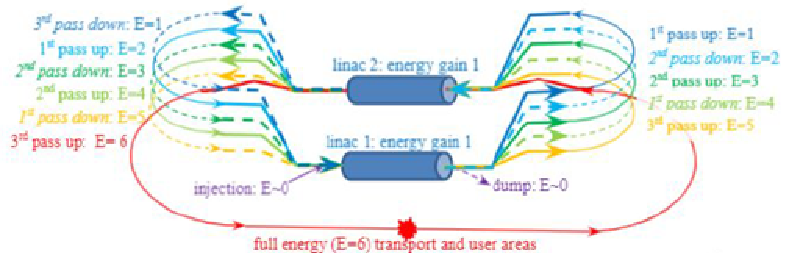
\includegraphics[width=0.8\textwidth]{Figures/DIANA_Inverse_Compton_Source_Design/DIANA_diagram_placeholder.pdf}
\caption{Drawing of the 3-turn DIANA ERL \textcolor{blue}{**PLACEHOLDER**}}
\label{fig:DIANA_ERL_diagram}
\end{figure}
Within the context of the wider accelerator community, this would be a national scale facility and is aligned to two projects in particular: a proposal for the UK-XFEL \cite{burnett2020uk} and as a solution for the Large Hadron--electron Collider (LHeC) \cite{valloni2013strawman,bruning2019exploring,holzer2021accelerator}. Within the wealth of accelerator solutions to a UK x-ray free electron laser presented in the UK-XFEL science case \cite{burnett2020uk}, a partial ERL solution is suggested with an ICS source. The UK-XFEL ICS source work is a precursor to the DIANA ICS source design as DIANA could be a potential demonstrator for the UK-XFEL. In terms of the LHeC project, the DIANA ERL could act as a proof-of-principle for the LHeC ERL alongside the existing PERLE accelerator \cite{angal2018perle}, demonstrating another design and transport approach.

High brilliance electron beams on the \si{\giga\electronvolt}-scale can facilitate applications such as a high power extreme ultraviolet (EUV) FEL and a $\gamma$-ray inverse Compton scattering source. An EUV FEL source would have far-reaching consequences for semiconductor lithography providing an unparalleled source of 13.5~\si{\nano\meter} EUV radiation (or some harmonic thereof). Whereas a narrowband $\gamma$-ray inverse Compton scattering source driven by an ERL would have considerable impact upon nuclear physics and security, beyond the achievements and opportunities available at storage ring facilities such as HI$\gamma$S \cite{weller2009research}. Within the scope of the authors current work, the focus is on the development of the latter application as well a progress toward a conceptual design of the DIANA ERL. Hence, the following chapter excludes EUV FEL developments.

A $\gamma$-ray ICS source at moderate energies ($E_{\gamma} < 5$~\si{\mega\electronvolt}) could enable applications such as nuclear resonance fluorescence (NRF) for inspection of nuclear fuel rods, waste studies and detection of clandestine nuclear material \cite{angell2015demonstration,bolind2015states} to high energy ($E_{\gamma} > 5$~\si{\mega\electronvolt}) applications such as nuclear photonics \cite{budker2021expanding} and medical isotope production \cite{habs2011production}. Here special consideration is given to the photo-nuclear production of medical isotopes. 

\section{Transport Optics Investigation}
\label{sec:DIANA_transport_optics_investigation}

\section{ERL ICS Electron Beam and Optical Cavity Laser Pulse Parameters}
\subsection{ERL ICS Electron Beam Parameters }
The electron bunch parameters for the DIANA ERL ICS are presented in Table~\ref{tab:DIANA_electron_beam_design_parameters}. Baseline parameters are designed for the case of a small interaction point $\beta$-function and therefore a small electron spot size in order to maximise the uncollimated flux and brilliance of the ICS source. This is also useful for highlighting changes within source performance that only occur due to the varying kinetic energy of the electron bunch. A non-round beam optimised case is also shown for maximising the collimated flux into a narrow 0.5\% bandwidth, which is optimised using the simplex non-round beam methodology in Chapter~\ref{Optimisation_and_Characterisation_of_Inverse_Compton Scattering_Spectra}. 

\begin{table}[H]
\centering
\caption{Electron beam parameters foreseen at the DIANA ICS source interaction point (IP). Baseline parameters assume a round transverse profile for the electron bunch whereas the optimised parameters are the result of a non-round beam optimisation \textcolor{blue}{what type?}. The given baseline parameters -- which assume the same $\beta^*$ at the IP -- allow a comparison of flux and bandwidth at different energies. The optimised values beneath those are designed to maximise the flux into a 0.5\% \textit{rms} scattered photon bandwidth through a trade-off of $\beta$-function of the electron bunch in each transverse plane and collimation angle.}
\begin{threeparttable}
\begin{tabular}{lccccc}
\hline\hline
Parameter & \multicolumn{3}{c}{Quantity} & Unit \\
\hline
Turn number & 1 & 2 & 3  \\
Injection Energy, $E_{\mathrm{inj}}$ & \multicolumn{3}{c}{7} & \si{\mega\electronvolt}\\
\tnote{$\dagger$}~Electron kinetic energy, $E_e$ & 362 & 717 & 1072 & \si{\mega\electronvolt}\\
Harmonic Frequency, $f$ & \multicolumn{3}{c}{125} & \si{\mega\hertz}\\
Bunch charge, $e N_e$ & \multicolumn{3}{c}{100} & \si{\pico\coulomb} \\
Beam current, $I$ & \multicolumn{3}{c}{12.5} & \si{\mill\ampere} \\
Transverse normalised \textit{rms} emittance, $\epsilon_{N}$ & \multicolumn{3}{c}{0.5} & \si{\milli\meter}-\si{\milli\radian}\\
\tnote{$\sharp$}~\textit{rms} bunch length, $\Delta \tau$ & \multicolumn{3}{c}{0.9 (3)} & \si{\milli\meter} (\si{\pico\second})\\
Bunch spacing, $t_{b}$ & \multicolumn{3}{c}{10} & \si{\pico\second} \\
RF frequency, $f_{RF}$ & \multicolumn{3}{c}{750} & \si{\mega\hertz} \\
\tnote{*}~Absolute energy spread, $\Delta E_{e}$ & \multicolumn{3}{c}{$\sim$10} & \si{\kilo\electronvolt} \\ 
\tnote{*}~Relative energy spread, $\left(\Delta E_{e}/E_{e}\right)$ & \multicolumn{3}{c}{$\sim10^{-5}$} & \\
\hline
\multicolumn{5}{c}{Baseline Parameters} \\
\hline
$\beta$-functions at the IP, $\beta_{x}^{*}$/$\beta_{y}^{*}$ & 0.2/0.2 & 0.2/0.2 & 0.2/0.2 & \si{\meter} \\
Electron bunch spot size, $\sigma_{e,x}$/$\sigma_{e,y}$ & 11.87/11.87 & 8.44/8.44 & 6.90/6.90 & \si{\micro\meter}\\
\hline\multicolumn{5}{c}{Optimised 0.5\% \textit{rms} Bandwidth} \\
\hline
$\beta$-functions at the IP $\beta_{x}^{*}$/$\beta_{y}^{*}$ & 1.33/0.298 & 2.62/0.587 & 3.90/0.874 & \si{\meter} \\
Electron bunch spot size, $\sigma_{e,x}$/$\sigma_{e,y}$ & 30.62/14.49 & 30.54/14.46 & 30.48/14.43 & \si{\micro\meter}\\
Collimation Angle, $\theta_{\mathrm{col}}$ & 0.180 & 0.091 & 0.061 & \si{\milli\radian} \\ 
\hline\hline
\end{tabular}
\begin{tablenotes}
\item[$\sharp$]{Taken from the ASML parameters.}
\item[*]{Estimated values.}
\item[$\dagger$]{Electron beam energies to accomplish $E_{\gamma}^{\mathrm{max}}$ = 20~\si{\mega\electronvolt} $\gamma$-rays. $\Delta E_{\mathrm{turn}}$ = 355~\si{\mega\electronvolt}.}
\end{tablenotes}
\end{threeparttable}
\label{tab:DIANA_electron_beam_design_parameters}
\end{table}

\subsection{Optical Cavity and Laser Pulse Parameters}

The envisioned parameters of the laser pulse provided by a Nd:YAG ($\lambda = 1064$~\si{\nano\meter}) laser and a four mirror Fabry-Perot optical cavity for use in the DIANA ICS source are shown in Table~\ref{tab:DIANA_laser_pulse_design_parameters}. Again, an Nd:YAG laser is selected for its picosecond domain and narrow spectral bandwidth. Only a single pulse is recirculated within the optical cavity which is designed to be operated with a fixed \textit{rms} laser pulse waist of radius 25~\si{\micro\meter}. A crossing angle of 5\si{\degree} must be imposed due to the geometry considerations of such a source.

These laser pulse parameters are based upon the demonstration of the Fabry-Perot optical cavity in the cERL ICS experiment \cite{akagi2016narrow}. However, they have been modified for a reduced 125~\si{\mega\hertz} repetition rate with an increased pulse energy of 100~\si{\micro\joule} resulting in an increased average stored power of 12.5~\si{\kilo\watt} recirculated in the optical cavity. Therefore, the parameters for the DIANA ICS source are slightly less conservative than those proposed for the CBETA ICS source in Table~\ref{tab:CBETA_laser_pulse_design_parameters} though the MuCLS demonstration of 70~\si{\kilo\watt} \cite{eggl2016munich} affords credibility to these design parameters.

\begin{table}[H]
\centering
\caption{Nd:YAG Gaussian laser pulse parameters at the CBETA ICS IP. The interacted laser pulse is produced via a Nd:YAG infrared laser and re-circulated in a bow-tie Fabry-Perot optical cavity.}
\begin{tabular}{lcc}
\hline\hline
Parameter & Quantity & Unit \\
\hline
Wavelength, $\lambda_\textrm{laser}$ & 1064 & \si{\nano\meter}\\
Photon energy, $E_\textrm{laser}$ & 1.17 & \si{\electronvolt}\\
Pulse energy, $E_{pulse}$  & 100 & \si{\micro\joule}\\
Number of photons, $N_{\textrm{laser}}$ & 5.34$\times 10^{14}$ & \\ 
Repetition rate, $f$ & 125 & \si{\mega\hertz}\\
Spot size at the IP, $\sigma_\textrm{laser}$ & 25 & \si{\micro\meter}\\
Crossing angle, $\phi$ & 5 & deg \\
Pulse length, $\tau_{\mathrm{laser}}$  & 10 & \si{\pico\second}\\
Relative energy spread, $\Delta E_\textrm{laser}/E_\textrm{laser}$ & $\times 10^{-5}$ &   \\
\hline\hline
\end{tabular}
\label{tab:DIANA_laser_pulse_design_parameters}
\end{table}

\section{ICS Source Spectral Output}

The anticipated spectral output of the DIANA ICS source, using the electron bunch and laser pulse parameters specified in Tables~\ref{tab:DIANA_electron_beam_design_parameters},~\ref{tab:DIANA_laser_pulse_design_parameters}, is presented in Table~\ref{tab:DIANA_spectral_output}. 

\begin{table}[H]
\centering
\begin{tabular}{lcccc}
\hline\hline
 & \multicolumn{3}{c}{Electron Kinetic Energy (\si{\mega\electronvolt})} & \\
 \cline{2-4}
 & 362 & 717 & 1072 & \\
\hline
$\gamma$-ray peak energy  & 2.33 & 9.06 & 20.11 & \si{\mega\electronvolt}\\
Source size ($x$/$y$)  & 10.72/10.72 & 8.00/8.00 & 6.65/6.65 & \si{\micro\meter} \\
Uncollimated flux  & 5.77$\times 10^{10}$ & 6.02$\times 10^{10}$ & 6.08$\times 10^{10}$ & ph/\si{\second}\\
Spectral density  & 2.48$\times 10^{5}$ & 6.65$\times 10^{4}$ & 3.03$\times 10^{4}$ & ph/\si{\second} \si{\electronvolt}\\
Average brilliance  & 5.64$\times 10^{12}$ & 2.05$\times 10^{13}$ & 4.45$\times 10^{13}$ & ph/\si{\second} \si{\milli\meter}$^{2}$\si{\milli\radian}$^{2}$ 0.1\% bw\\
Peak brilliance  & 5.60$\times 10^{17}$ & 2.22$\times 10^{18}$ & 4.99$\times 10^{18}$ & ph/\si{\second} \si{\milli\meter}$^{2}$ \si{\milli\radian}$^{2}$ 0.1\% bw\\
\hline
 & \multicolumn{3}{c}{0.5\% \textit{rms} bandwidth} & \\
\hline
Source Size ($x$/$y$) & 19.36/12.54 & 19.35/12.52 & 19.33/12.50 & \si{\micro\meter} \\ 
Collimated flux  & 1.30$\times 10^{9}$ & 1.29$\times 10^{9}$ & 1.29$\times 10^{9}$ & ph/\si{\second} 0.5\% bw \\
\hline\hline
\end{tabular}
\label{tab:DIANA_spectral_output}
\end{table}

\begin{figure}[!h]
\centering
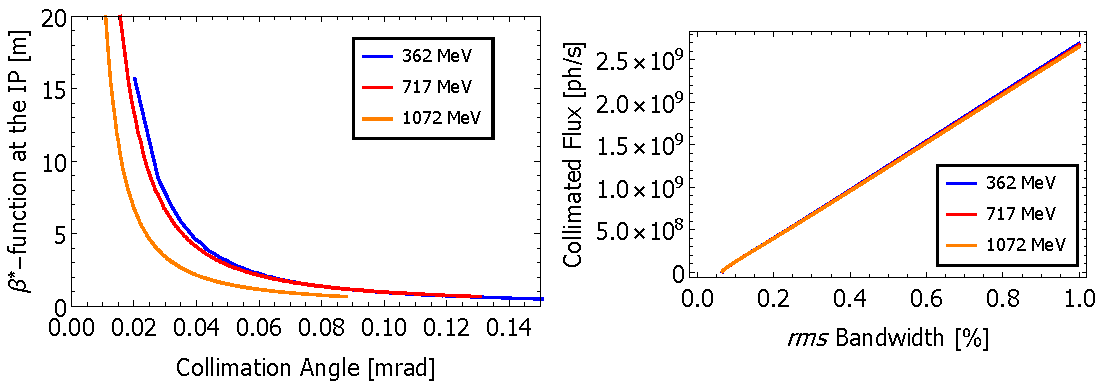
\includegraphics[width=\textwidth]{Figures/DIANA_Inverse_Compton_Source_Design/DIANA_Tuning_Curve_Opt/DIANARBplot.pdf}
\caption{Round beam optimisation comparison at the three nominal energies 362~\si{\mega\electronvolt} (blue), 717~\si{\mega\electronvolt} (red), 1072~\si{\mega\electronvolt} (orange) of the DIANA ICS source. Left: Optimised tuning curves of the $\beta^{*}$-function at the IP (same in both planes) against the collimation angle for each nominal electron energy. Right: collimated flux as a function of the \textit{rms} bandwidth of the DIANA ICS source at each nominal energy.}
\label{fig:DIANA_RB_comparison}
\end{figure}

\begin{figure}[!h]
\centering
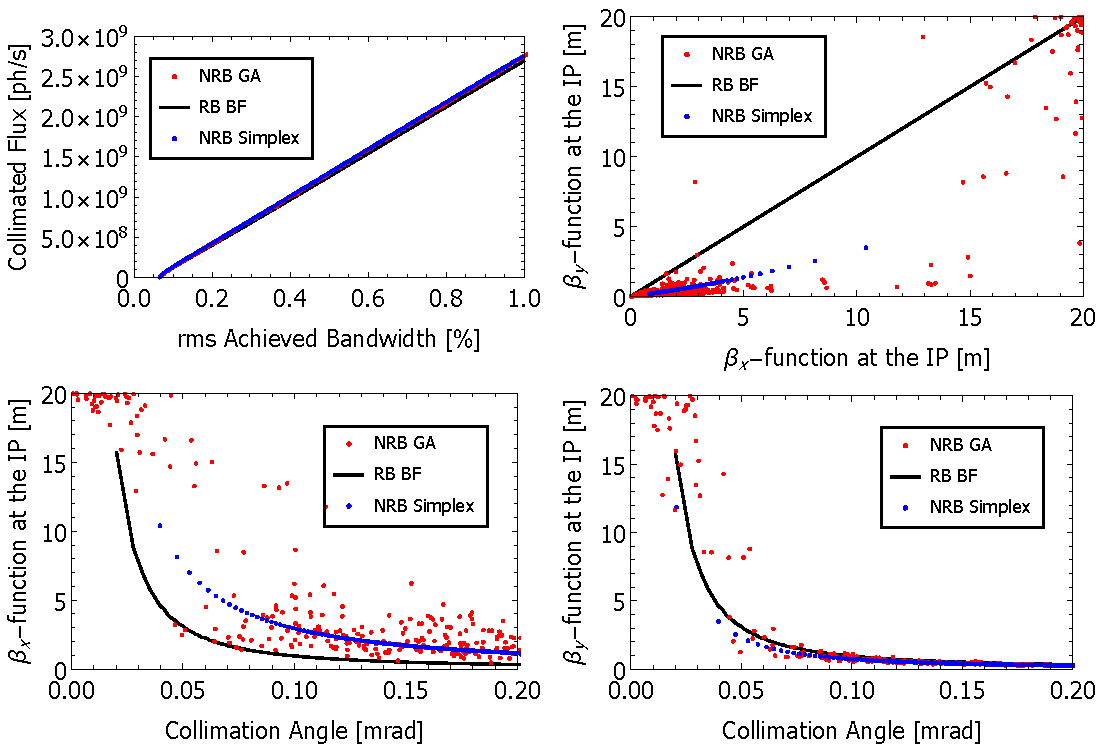
\includegraphics[width=\textwidth]{Figures/DIANA_Inverse_Compton_Source_Design/DIANA_Tuning_Curve_Opt/DIANA362fullcomp.pdf}
\caption{DIANA 362~\si{\mega\electronvolt} 1st turn ICS source optimisations, comparing the two non-round beam approaches (simplex and GA) and the round beam approach. Top Left: collimated flux as a function of \textit{rms} bandwidth pareto fronts of the source. Top Right: interaction point $\beta$-function parameter space in the $x$ and $y$ plane for optimised cases. Bottom Left: parameter space of the interaction $\beta$-function in the $x$ plane and collimation angle for optimised cases. Bottom Right: parameter space of the interaction $\beta$-function in the $y$ plane and collimation angle for optimised cases.}
\label{fig:DIANA362_comparison_optimisation}
\end{figure}

\begin{figure}[!h]
\centering
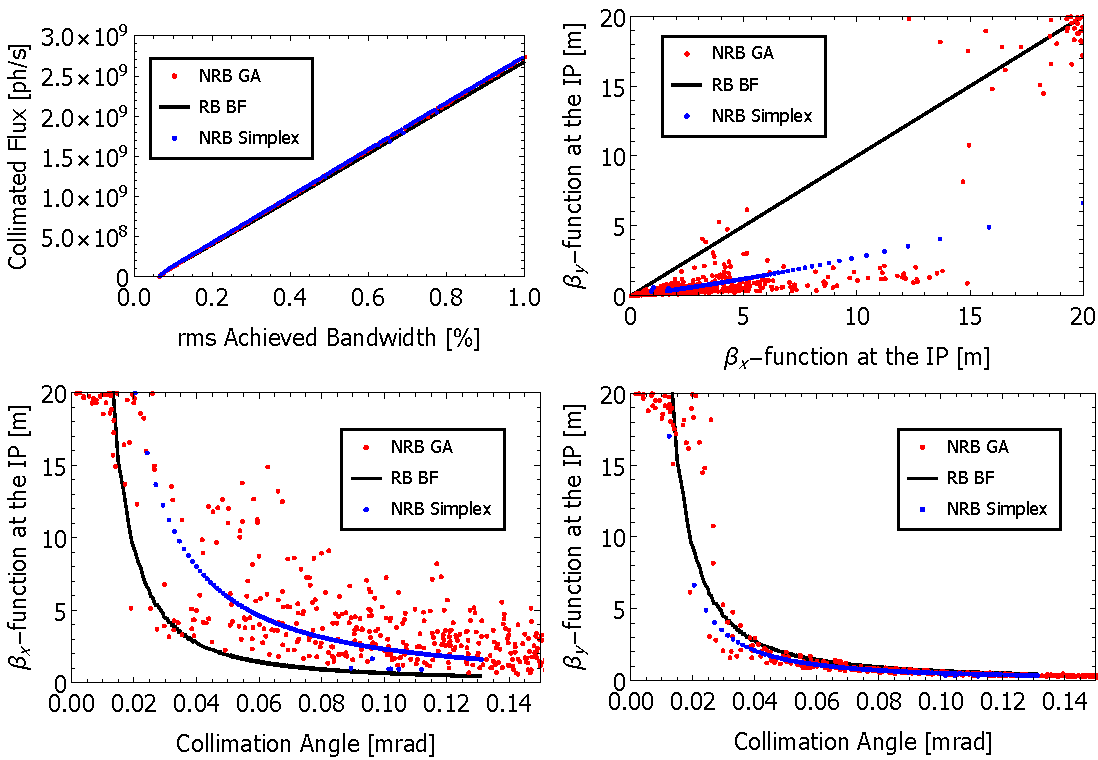
\includegraphics[width=\textwidth]{Figures/DIANA_Inverse_Compton_Source_Design/DIANA_Tuning_Curve_Opt/DIANA717fullcomp.pdf}
\caption{DIANA 717~\si{\mega\electronvolt} 2nd turn ICS source optimisations, comparing the two non-round beam approaches (simplex and GA) and the round beam approach. Top Left: collimated flux as a function of \textit{rms} bandwidth pareto fronts of the source. Top Right: interaction point $\beta$-function parameter space in the $x$ and $y$ plane for optimised cases. Bottom Left: parameter space of the interaction $\beta$-function in the $x$ plane and collimation angle for optimised cases. Bottom Right: parameter space of the interaction $\beta$-function in the $y$ plane and collimation angle for optimised cases.}
\label{fig:DIANA717_comparison_optimisation}
\end{figure}

\begin{figure}[!h]
\centering
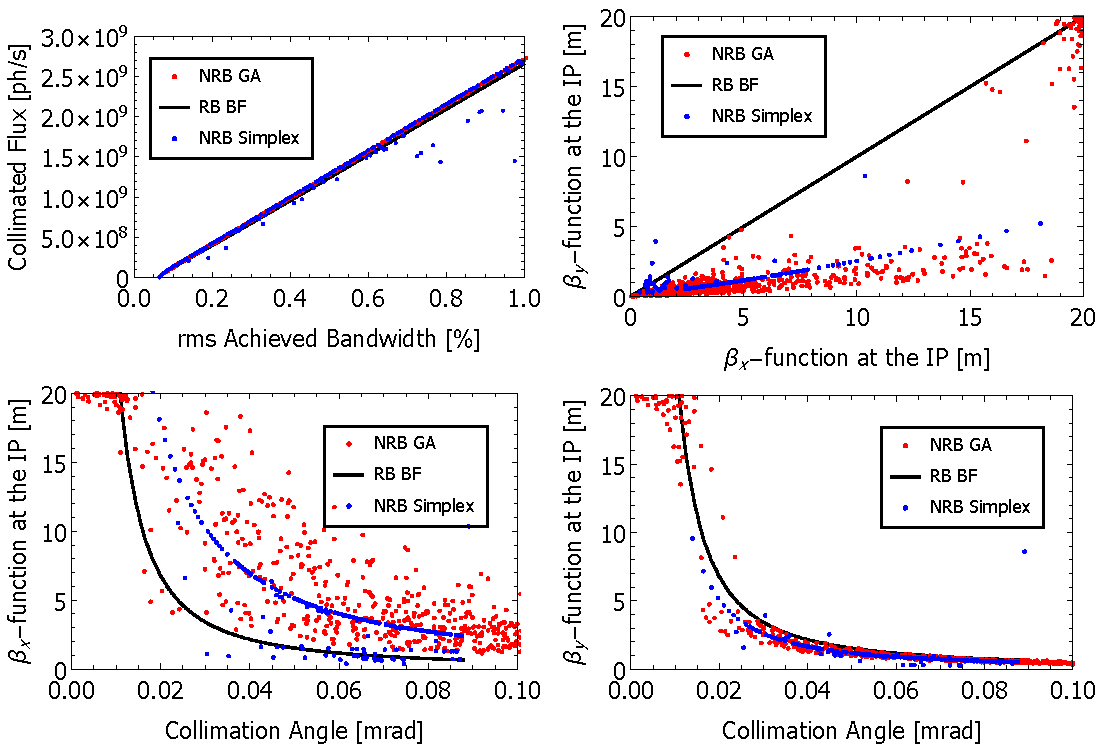
\includegraphics[width=\textwidth]{Figures/DIANA_Inverse_Compton_Source_Design/DIANA_Tuning_Curve_Opt/DIANA1072fullcomp.pdf}
\caption{DIANA 1072~\si{\mega\electronvolt} 3rd turn ICS source optimisations, comparing the two non-round beam approaches (simplex and GA) with the round beam approach. Top Left: collimated flux as a function of \textit{rms} bandwidth pareto fronts of the source. Top Right: interaction point $\beta$-function parameter space in the $x$ and $y$ plane for optimised cases. Bottom Left: parameter space of the interaction $\beta$-function in the $x$ plane and collimation angle for optimised cases. Bottom Right: parameter space of the interaction $\beta$-function in the $y$ plane and collimation angle for optimised cases.}
\label{fig:DIANA1072_comparison_optimisation}
\end{figure}

\section{$\gamma$-ray ICS Source Comparison}

Inverse Compton scattering sources for production of $\gamma$-rays have been developed and designed worldwide. Differing approaches for the production of $\gamma$-rays have been trialed such as variations on the type of accelerators and incident photon sources used. For example, the HI$\gamma$S source uses radiation produced from a free electron laser to achieve high energy photon production up to 100~\si{\mega\electronvolt}. The most relevant facilities for comparison to the DIANA ICS are tabulated in Table~\ref{tab:gammaray_ICS_comparison}, this presents a combination of operating facilities and recently designed sources. 

\begin{table}[!h]
\caption{Comparison of existing and designed $\gamma$-ray ICS.}
\begin{threeparttable}
\begin{tabular}{lccc}
\hline\hline
ICS & Accelerator Type & Scattered Photon Energy (\si{\mega\electronvolt}) & Flux (ph/\si{\second}) \\
\hline
DIANA\tnote{*} & ERL & 2.33--20.11 & 5.77--6.08$\times 10^{11}$ \\ 
NIJI-IV \cite{sei2017demonstration} & Storage Ring & 1.2 & 3.1$\times 10^{4}$ \\ 
ELI-NP-GBS\tnote{*} \cite{adriani2014technical} & Linac & 0.2--19.5 & $3.9\times 10^{9}$ \\
ELI-NP VEGA\tnote{*} \cite{tanaka2020current,elinp2019vega} & Storage Ring & 1--19.5 & 1$\times 10^{11}$\\
NewSUBARU \cite{utsunomiya2015gamma} & Storage Ring & 5--40 & $3\times 10^{7}$ \\
%VELOCIRAPTOR & Linac & & \\
%T-REX & Linac & & \\
Pan et al CBS\tnote{*} \cite{pan2019design} & Storage Ring & 4--10 & 0.14--3.87$\times 10^{12}$ \\ 
Super-ACO \cite{nutarelli1998gamma} & Storage Ring & 13 & $5\times10^{6}$ \\
HI$\gamma$S\tnote{$\dagger$} ~\cite{weller2009research} & Storage Ring & 1--100 & 5$\times 10^{7}$--5$\times 10^{8}$ \\
\hline\hline
\end{tabular}
\begin{tablenotes}
\item[*]{Denotes design parameters for sources which are not yet demonstrated.}
\item[$\dagger$]{The HI$\gamma$S source is capable of scattered photon energies up to 100~\si{\mega\electronvolt}. }
\end{tablenotes}
\end{threeparttable}
\label{tab:gammaray_ICS_comparison}
\end{table}

As is evident from Table~\ref{tab:gammaray_ICS_comparison}, in-depth consideration of an ERL as the driver of an inverse Compton scattering source for production of $\gamma$-rays is limited. Predominantly ICS $\gamma$-ray production is driven by storage ring methods with the existing facilities such as NewSUBARU and HI$\gamma$S sources utilising existing synchrotron facilities. 

\section{Bremsstrahlung Source Comparison}

\section{DIANA ICS Applications}
\textcolor{blue}{**$\gamma$-ray applications from CBETA** \\ **SOME MAY BE USEFUL**}

The final ambitious application, nuclear resonance fluorescence (NRF), is a technique suitable for a future, higher-energy ERL based ICS, with an electron beam energy on the order of 350~\si{\mega\electronvolt} or above. This electron beam energy regime boosts the Compton back scattered photons into the regime of gamma rays with an energy of 2.2~\si{\mega\electronvolt} or above. These in turn would be used to excite nuclear levels identifying them with a energy sensitive solid state detector, achieving the nuclear sister spectroscopy to the atomic fluorescence spectroscopy mentioned in our first application. Such spectroscopy would be very useful in assaying nuclear materials, for example identification of manufacturing defects in fission fuel assemblies, nonproliferation security of spent fission fuel and identification of unknown legacy wastes~\cite{angal2018perle,angell2015demonstration,bolind2015states,geddes2017impact,kwan2011discrete}. Moving up to photon energies above $5$~\si{\mega\electronvolt} (requiring a \si{\giga\electronvolt}-scale electron ERL) would open up the nuclear transmutation reactions $(\gamma,p)$, $(\gamma,n)$, $(\gamma,f)$ with potentially far-reaching applications in waste transmutation \cite{ur2017optimization}, the understanding of fission dynamics \cite{bellia1983towards,bhike2017exploratory,finch2018monoenergetic} and bespoke medical isotope production from existing waste streams \cite{habs2011production}. 

\end{document}